\documentclass[12pt,convert={false}]{standalone}
\usepackage[dvipsnames]{xcolor}
\usepackage{tikz}
\usetikzlibrary{shapes,arrows,positioning,calc,patterns,arrows.meta, bending, graphs, shadings,quotes,intersections}
\usetikzlibrary{external}
%\tikzexternalize[prefix=tikz/]
\usepackage{pgfplots}
\pgfplotsset{compat=1.16}
\usepgfplotslibrary{fillbetween}
\newcommand{\enf}[1]{\textcolor{RedViolet}{\textbf{#1}}} %enf sta per enfasi
\newcommand{\sott}[1]{\setulcolor{black!20!Goldenrod}\ul{#1}}
\newcommand{\prob}{\mathbb{P}}
\newcommand\independent{\protect\mathpalette{\protect\independenT}{\perp}}
\newcommand{\ev}[1]{\mathbb{E}\Bigl[{#1}\Bigr]}
\def\independenT#1#2{\mathrel{\rlap{$#1#2$}\mkern2mu{#1#2}}}
\newcommand{\Z}{\mathbb{Z}}
\newcommand{\R}{\mathbb{R}}
\newcommand{\N}{\mathbb{N}}
\newcommand{\equalexpl}[1]{%
	\underset{\substack{\uparrow\\\mathrlap{\text{\vspace{-3cm}\hspace{-1em}#1}}}}{=}}
\newcommand{\dif}{\mathop{}\!\mathrm{d}}
\begin{document}
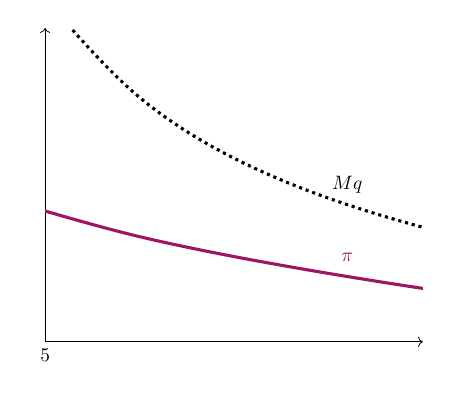
\begin{tikzpicture}[scale=0.7]
	\begin{axis}[
		xlabel=\empty,
		x axis line style={->,opacity=100},
		ylabel=\empty,
		xmin=5, xmax=10,
		ymin=0, ymax=1,
		axis y line=left,
		y axis line style={->,opacity=100},
		ytick={1.4487},
		xtick={5},
		xticklabels={5},
		yticklabels={$\phi(5)$},
		axis x line*=bottom
		]
		\addplot[domain=0:150, RedViolet, ultra thick,smooth] {e^(-x*0.1)-0.2};
		\addplot[domain=0:150, black, ultra thick,smooth,dotted] {e^(-x*0.2+1)};
		\node[align=left] at (9,0.5) {$Mq$};
		\node[align=left, RedViolet] at (9,0.27) {$\pi$};
	\end{axis}
\end{tikzpicture}
\end{document}
